\section{Introduction}

%---------------------------------------------------------

\subsection{Convolutional Neural Networks (CNN)}

\begin{frame}
\frametitle{Convolutional Neural Networks (CNN)}
\begin{columns}
\begin{column}{0.5\textwidth}
In deep learning, a \textbf{Convolutional Neural Network (CNN)} is a class of deep neural networks, most commonly applied to analyzing visual imagery.

\vspace{0.5cm}
A convolutional neural network consists of an input and an output layer, as well as multiple hidden layers, they are

\begin{itemize}
    \item Convolutional Layer
    \item Pooling Layer
    \item Fully-connected Layer
\end{itemize}
\end{column}

\begin{column}{0.5\textwidth}
\begin{figure}
    \centering
    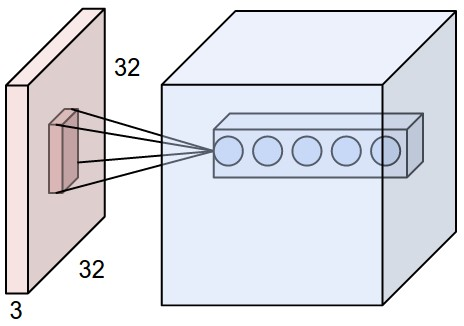
\includegraphics[width=\textwidth]{conv}
    \caption{An example of convolutional layer \footnotemark.}
\end{figure}
\end{column}
\end{columns}

\footnotetext{\url{http://cs231n.github.io/convolutional-networks/}}
\end{frame}


\begin{frame}
\vspace{-0.5cm}
\frametitle{Solutions and Performance}
{
\tiny{
\begin{longtable}[]{@{}l|l|l|l|l|l|l@{}}
\caption{Summary of Solutions to Challenges and Performance on PASCAL VOC 2012 Challenge \citep{Everingham2010} within Each Method Reviewed.}
\label{tab:summary}
\\
\hline
Challenges & \begin{tabular}[c]{@{}l@{}}Reduced \\ Features \\ Resolution\end{tabular} & \begin{tabular}[c]{@{}l@{}}Global \\ Context \end{tabular} & \begin{tabular}[c]{@{}l@{}}Limited \\ Receptive \\ Fields\end{tabular} & \begin{tabular}[c]{@{}l@{}}Spatial \\ Invariance  \end{tabular}& \begin{tabular}[c]{@{}l@{}}Boundary \\ Recovery \end{tabular} & \begin{tabular}[c]{@{}l@{}}VOC 2012 \\ mean IU\end{tabular}\tabularnewline
\hline
\endhead
FCN & \begin{tabular}[c]{@{}l@{}}Upsampling \\ through \\ bilinear \\ interpolation\end{tabular} & \(\times\) &
\begin{tabular}[c]{@{}l@{}}Aggregation \\ of \\ low-level \\ features\end{tabular} & \(\times\) & \begin{tabular}[c]{@{}l@{}}Aggregation \\ of \\ low-level \\ features\end{tabular} & 67.2\tabularnewline
\hline
PSPNet & \begin{tabular}[c]{@{}l@{}}Upsampling \\ through \\ deconvolution\end{tabular} & \begin{tabular}[c]{@{}l@{}}Global \\ average \\ pooling\end{tabular} &
\begin{tabular}[c]{@{}l@{}}Region-\\based \\ pooling\end{tabular} & \(\times\) & \(\times\) & 85.4\tabularnewline
\hline
U-Net & \begin{tabular}[c]{@{}l@{}}Upsampling \\ through \\ deconvolution\end{tabular} & \(\times\) & \(\times\) &
\(\times\) & \begin{tabular}[c]{@{}l@{}}Encoder-\\decoder \end{tabular} & \(\times\)\tabularnewline
\hline
DeepLab v2 & ASPP & \(\times\) & ASPP & CRF & \(\times\) &
79.7\tabularnewline
\hline
DeepLab v3 & ASPP & \begin{tabular}[c]{@{}l@{}}Global \\ average \\ pooling\end{tabular} & ASPP & \(\times\) &
\(\times\) & 86.9\tabularnewline
\hline
DeepLab v3+ & ASPP & \begin{tabular}[c]{@{}l@{}}Global \\ average \\ pooling\end{tabular} & ASPP & \(\times\) &
\begin{tabular}[c]{@{}l@{}}Encoder-\\decoder \end{tabular} & 89.0\tabularnewline
\end{longtable}
}
}
\pause
\begin{enumerate}
    \item DeepLab aggregates great ideas from other methods along its way.
    \pause
    \item DeepLab v3+ achieves the best performance.
    \pause
    \item The more challenges are addressed, the higher performance is.
\end{enumerate}
\end{frame}


%---------------------------------------------------------

